\section{Introduction}
\begin{frame}{Motivation}
\begin{columns}
\column{0.5\textwidth}
\begin{itemize}
\item Many challenges exist regarding modern combustion systems 
\item Better modeling can improve performance, efficiency, and reliability 
\item Detonation engines are a growing area of interest 
\item Current CFD models are computationally expensive
\item Adaptive meshing can reduce computational expense
\end{itemize}	

\column{0.5\textwidth}
\begin{figure}
\centering
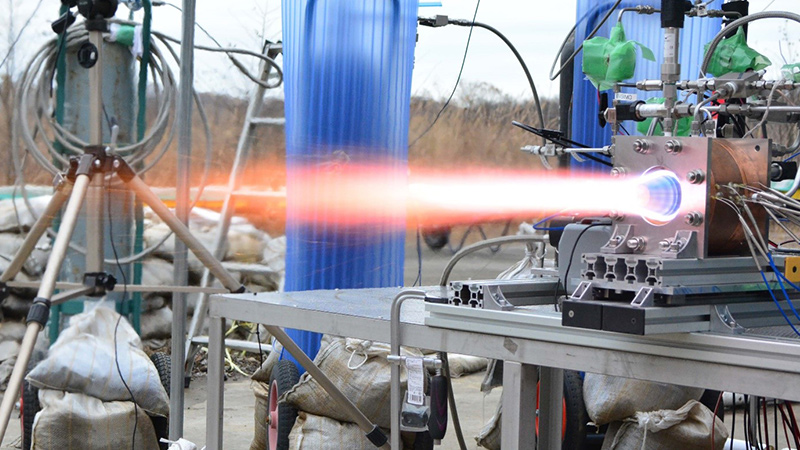
\includegraphics[width=\textwidth]{../figs/rde.jpg}
\caption{Nagoya University 900 N Rotating Detonation Engine \cite{nagoya}}
\end{figure}
\end{columns}
\end{frame}

\begin{frame}{Objectives}
\begin{itemize}
\item Implement and test AMR techniques for simulations of detonations found within RDEs and PDEs within OpenFOAM \cite{weller}, which has:
\begin{itemize}
\item geometric flexibility 
\item consistent input structure (easy to transition between solvers)
\item good documentation
\item open source, GNU GPL
\end{itemize}
\item Build a framework on previous work by Towery \cite{towery1} and TESLa at CU Boulder for further RDE and PDE research 
\end{itemize}
\end{frame}

\begin{frame}{Previous Work}
    
\end{frame}
